\subsection{Simplification: the input decides, not the UVs}
\label{sec:simplification}

\begin{figure}[t]
\centering
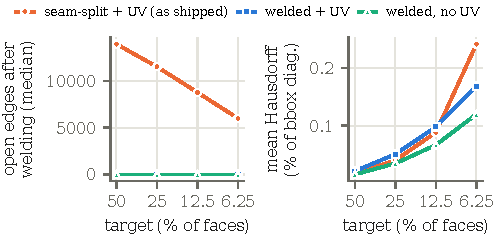
\includegraphics[width=\columnwidth]{figures/decimation}
\caption{Simplifying the 24 raw assets (medians). Left: boundary edges in the
output, counted after welding identical positions; the inputs have none.
Seam-split input cracks at every target; welded input, with or without UVs,
never does (the two lines coincide at zero). Right: mean surface distance to
the original.}
\Description{Two line charts over four simplification targets. Left: the
seam-split line falls from about 14,000 to 6,000 boundary edges; the welded lines
stay at zero. Right: mean distance rises for all three inputs, from about 0.02 to
0.24 percent of the bounding-box diagonal.}
\label{fig:decimation}
\end{figure}

\begin{table}[t]
\caption{Simplification at 6.25\,\% of the triangles (24 assets, up to three
passes). Distance: mean surface distance, \% of the bounding-box diagonal,
median [max]. Colour: base-colour RMSE above the unsimplified noise floor
(0--255 scale), median [max]. The maxima for W both come from the asset that
stalled. $^{*}$Normal preservation on; with it off, as for S and W, all 24 also
reach the target with no cracks.}
\label{tab:decimation}
\small
\begin{tabularx}{\columnwidth}{@{}Yrrrr@{}}
\toprule
Input & Reached & Cracked & Distance & Colour \\
\midrule
S: seam-split + UV & 18 & 24 & 0.24 [0.32] & 3.5 [9.6] \\
S, boundary preserved & 0 & 0 & -- & 2.4 [16.7] \\
W: welded + UV & 23 & 0 & 0.17 [1.40] & 3.7 [37.1] \\
N: welded, no UV$^{*}$ & 24 & 0 & 0.12 [0.20] & -- \\
\bottomrule
\end{tabularx}
\end{table}

H4 is not supported. Welded and with UVs preserved, 23 of 24 assets reached
6.25\,\% of their triangles (about 3,100) in one pass with no cracks
(Table~\ref{tab:decimation}). The exception has the most UV charts (3,088) and
stalled at 3,800--3,900 triangles after three passes (two runs). Charts constrain where the
simplifier may collapse, but at these budgets they rarely stop it.

What decided the outcome was the input. MeshLab's glTF loader returns the
file's seam-split buffer, in which every UV seam already separates the surface
into distinct vertices, as glTF requires~\cite{khronos2021gltf}. MeshLab's
texture-aware simplification then treats each seam as an open boundary. With
boundary preservation off (the default) the two sides of every seam move
independently: every asset cracked at every target, with a median of 13,924 open
edges already at 50\,\% (Figure~\ref{fig:decimation}), and six assets did not
reach 6.25\,\% within three passes. With boundary preservation on, nothing cracks
but nothing gets far: no asset went below 13,238 triangles, and the median stopped
at 21,939, about 44\,\% of the original. The filter reports no error in either
case. The failure depends on the tool. meshoptimizer, which infers seams from
matching positions~\cite{meshopt}, did not crack the same seam-split inputs but
stalled: two of 24 reached 6.25\,\% (median 5,900 triangles), against 24 of 24 on
welded input.

Welding identical positions first removes the problem in both tools; in
PyMeshLab this is one call, \texttt{meshing\_remove\_\allowbreak duplicate\_\allowbreak vertices},
which keeps UVs per corner. The
cost in colour is modest: median base-colour error above the noise floor is
1.5 levels at 12.5\,\% (0.1 for seam-split input) and 3.7 at 6.25\,\% (3.5), on a
0--255 scale, with one outlier at 37 for the asset that stalled. Mean surface
distance is slightly higher than for seam-split input at 50--12.5\,\% and lower at
6.25\,\%. Attribute discontinuities are a classic concern in
simplification~\cite{hoppe1996pm,hoppe1999newqem}, and the weld-first rule is
documented~\cite{meshopt}; what this case shows is how silently a common scripted
path runs into them.

This is what happened to the companion. Our pipeline loaded the 497,850-triangle
GLB directly and simplified it in three passes to 82,829 triangles, giving the
torn mesh of Section~\ref{sec:hygiene} (Figure~\ref{fig:assets}, bottom). The
design note for that step says the simplifier stopped near 106k triangles
because the UV islands were a hard floor. That figure came from an earlier trial
run; the shipped script multiplies the target by 0.55 per pass and simply ran its
three passes ($497{,}850 \times 0.55^3 \approx 82{,}830$). On the welded input the
same filter takes the companion to 31,116 triangles (6.25\,\%) in one pass with
no boundary edges. The torn mesh shipped after a play check recorded only as
``Play-verified'' in the commit history.
